
\textbf{Le but de ce projet est de construire numériquement un modem} (modulateur-démodulateur). \\
A fin de tester nos compétences acquises en traitement du signal numérique, nous devons coder un modem 
de fréquence en matlab.
Un signal numérique binaire est transmis via un canal de transmission virtuel après avoir été modulé en 
fréquence. Lors de cette transmission un bruit est ajouté. Le but est donc de démoduler le signal en
sortie du canal, et de le traiter afin de retrouver le message initial, malgré le bruit.

Dans une première partie le traitement du bruit se fera à l'aide d'un filtre, puis nous implémenterons 
la recommandation V21 de l’Union Internationale des Télécommunications (c.f. Annexe A).

\begin{figure}[ht!]
   \centering
   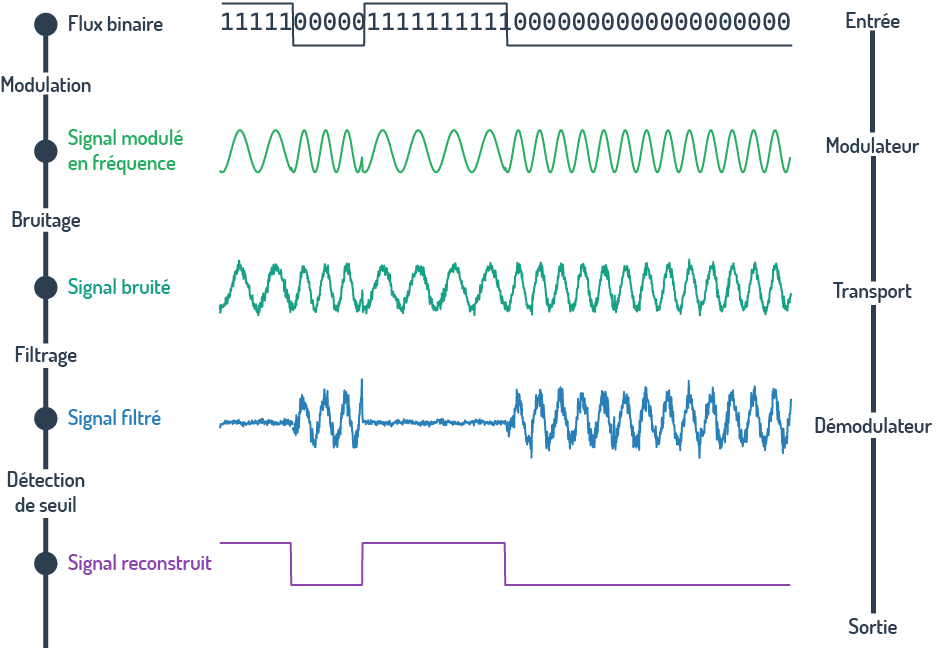
\includegraphics[scale=0.4]{partie-1/sous-partie-1/but}
   \caption{Principe du projet \label{fig : principe_projet}}
\end{figure}